\begin{frame}{What a Long Context Is For}
  \begin{itemize}\itemsep0.45em
    \item[\textcolor{red}{$\blacktriangleright$}] Many real inputs do not fit in a few thousand tokens: a code repository and the issue filed against it, a contract or a book, hours of transcribed audio, and the trace an agent accumulates as tool calls pile up.
    \item[\textcolor{red}{$\blacktriangleright$}] Context windows have grown from 2K tokens to 128K and beyond. The Gemini~1.5 report goes further: \textbf{near-perfect retrieval (\textgreater 99\%) up to at least 10M tokens} in its experiments.
    \item[\textcolor{red}{$\blacktriangleright$}] A long window lets a model use material it was never trained on. Given a grammar manual for Kalamang, a language with fewer than 200 speakers, Gemini~1.5 translated English to Kalamang at a level similar to a person who learned from the same materials.
    \item[\textcolor{red}{$\blacktriangleright$}] The window is a capacity, and an expensive one. Three questions organise this lecture: what a long context costs, how much of it a model actually uses, and which techniques make long inputs affordable.
  \end{itemize}
  \vspace{0.2em}
  {\scriptsize Gemini Team, Google, ``Gemini 1.5: Unlocking Multimodal Understanding Across Millions of Tokens of Context,'' 2024, \href{https://arxiv.org/abs/2403.05530v5}{arXiv:2403.05530v5}, abstract.}
\end{frame}

\begin{frame}{Three Costs That Grow With Length}
  \begin{columns}[T,onlytextwidth]
    \column{0.54\textwidth}
      \begin{itemize}\footnotesize\itemsep0.35em
        \item[\textcolor{red}{$\blacktriangleright$}] \textbf{Compute.} Over a causal sequence of $n$ tokens, attention costs about $2n^2d$ FLOPs per layer and the weight matrices $2nP$ ($d$: model width, $P$: parameters per layer). Attention dominates once $n > P/d$.
        \item[\textcolor{red}{$\blacktriangleright$}] \textbf{Memory.} The KV cache holds a key and a value per token, layer and KV head:
          \[ \text{bytes} = 2 \cdot L \cdot h_{kv} \cdot d_h \cdot (\text{bytes per value}) \cdot n, \]
          for $L$ layers and $h_{kv}$ KV heads of dimension $d_h$. It is linear in $n$ and kept per request.
        \item[\textcolor{red}{$\blacktriangleright$}] \textbf{Use.} Positions past the training length are out of distribution (RoPE rescaling), and models under-use even trained positions.
        \item[\textcolor{red}{$\blacktriangleright$}] Llama~3 trains on long sequences last because ``the compute in self-attention layers grows quadratically in the sequence length.''
      \end{itemize}
    \column{0.44\textwidth}
      \centering
      {\footnotesize Worked example: Llama~3.1~8B}\\[0.3em]
      {\scriptsize
      \begin{tabular}{rrr}
        \toprule
        $n$ (tokens) & KV cache & attention / weights \\
        \midrule
        8,192 & 1\,GiB & 0.15 \\
        32,768 & 4\,GiB & 0.62 \\
        131,072 & 16\,GiB & 2.46 \\
        1,048,576 & 128\,GiB & 19.7 \\
        \bottomrule
      \end{tabular}\par}
      \vspace{0.4em}
      \begin{itemize}\scriptsize\itemsep0.15em
        \item $L = 32$, $h_{kv} = 8$, $d_h = 128$, $d = 4096$, FFN width 14,336, bf16.
        \item $2 \cdot 32 \cdot 8 \cdot 128 \cdot 2 = 131{,}072$ bytes: 128\,KiB per token, so one 128K-token request needs 16\,GiB, about the size of the bf16 weights.
        \item $P \approx 218$ million parameters per layer, so $P/d = 53{,}248$ tokens.
      \end{itemize}
  \end{columns}
  \vspace{0.1em}
  {\scriptsize Llama Team, AI @ Meta, ``The Llama 3 Herd of Models,'' 2024, \href{https://arxiv.org/abs/2407.21783v3}{arXiv:2407.21783v3}, Table~3 and Section~3.4.2; table values computed from that configuration.}
\end{frame}

\begin{frame}{Three Families of Techniques}
  \centering
  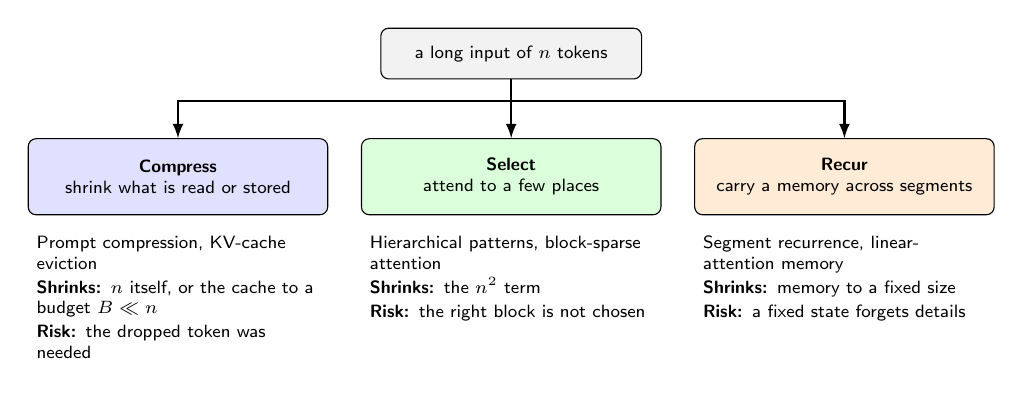
\begin{tikzpicture}[font=\sffamily\scriptsize, >=latex, scale=0.92,
      every node/.style={transform shape},
      fam/.style={draw, rounded corners=0.1cm, align=center, text width=3.9cm, minimum height=1.05cm},
      det/.style={align=left, text width=3.9cm, font=\sffamily\scriptsize},
      src/.style={draw, rounded corners=0.1cm, fill=gray!10, align=center, minimum width=3.6cm, minimum height=0.7cm}]
    \node[src] (input) at (0,2.7) {a long input of $n$ tokens};
    \node[fam, fill=blue!12] (comp) at (-4.6,1.0) {\textbf{Compress}\\shrink what is read or stored};
    \node[fam, fill=green!14] (sel) at (0,1.0) {\textbf{Select}\\attend to a few places};
    \node[fam, fill=orange!16] (rec) at (4.6,1.0) {\textbf{Recur}\\carry a memory across segments};
    \draw[->, thick] (input.south) -- ++(0,-0.3) -| (comp.north);
    \draw[->, thick] (input.south) -- (sel.north);
    \draw[->, thick] (input.south) -- ++(0,-0.3) -| (rec.north);
    \node[det, anchor=north] at (-4.6,0.3) {Prompt compression, KV-cache eviction\\[0.2em]\textbf{Shrinks:} $n$ itself, or the cache to a budget $B \ll n$\\[0.2em]\textbf{Risk:} the dropped token was needed};
    \node[det, anchor=north] at (0,0.3) {Hierarchical patterns, block-sparse attention\\[0.2em]\textbf{Shrinks:} the $n^2$ term\\[0.2em]\textbf{Risk:} the right block is not chosen};
    \node[det, anchor=north] at (4.6,0.3) {Segment recurrence, linear-attention memory\\[0.2em]\textbf{Shrinks:} memory to a fixed size\\[0.2em]\textbf{Risk:} a fixed state forgets details};
  \end{tikzpicture}\\[0.8em]
  \begin{itemize}\footnotesize\itemsep0.3em
    \item[\textcolor{red}{$\blacktriangleright$}] Each family trades exactness for cost in a different place. The lecture first measures how much context models really use, then takes the three families in turn and ends with how to choose between them and retrieval.
  \end{itemize}
\end{frame}
